\documentclass[a4paper, 11pt]{article}

\usepackage{hyperref}
\voffset -0cm
\hoffset 0.0cm
\textheight 23cm
\textwidth 16cm
\topmargin 0.0cm
\oddsidemargin 0.0cm
\evensidemargin 0.0cm

\usepackage{epsfig}
\usepackage{setspace}
\usepackage{fancyheadings}
\usepackage{amsmath}
\usepackage{amssymb}
\usepackage{graphicx}
\usepackage{url}

\title{}
\author{}
\date{}

\begin{document}

\begin{center}
	\LARGE \textbf{TD11: Discrete Capacity-Constrained Voronoi Tessellation}
\end{center}

\bigskip
\par In this TP, the objective is to implement a point sampling
strategy from a variant of Voronoi diagram: the capacity-constrained
Voronoi diagram
\cite{BalzerHeck:2008:CCVDIFS,Balzer.etal:2009:CCPDAVoLM}.

The main idea is to optimize a Voronoi diagram (by moving sites) such
that each Voronoi cell have the same area (capacity).  The digital
version can be described as follows: we want to sample $n$ points in a
$N\times N$ domain. Hence, each cell will be represented by a label
$l\in\{1\ldots n\}$. The problem is thus to distribute labels to
pixels in the $N\times N$ domain.

The first version of the algorithm can be sketched as follows:

\begin{enumerate}
\item First, each pixel randomly picks its label $l$ such that the
  number of pixels with label $l$ is  $\frac{N^2}{l}$;
\item To each label $l$, $C_l$ denotes the centroid of points with
  label $l$;

\item Until stability
  \begin{itemize}
  \item Randomly select a pair of points $p$ and $q$ with
    labels $l_p$ and $l_q$ ($l_p\neq l_q$);
  \item If swapping the labels of $p$ and $q$ \textbf{decreases the
    energy}, we perform the swap  ($l_p\leftrightarrow l_q$) and
    update the centroids $C_{l_p}$ and $C_{l_q}$;
  \end{itemize}
\end{enumerate}

The global energy to minimize is related to a ``Voronoi-like''
energy. In this simple digital setting, we just need to check is
swapping the label reduces the distances between the points and their
new cluster centroids.
More formally, we define
\begin{displaymath}
  \Delta e(p,l_p,l_q) = \|p-C_{l_p}\|^2 - \|p-C_{l_q}\|^2
\end{displaymath}
as the energy difference when the change the label of $p$ from $l_p$
to $l_q$. We perform the swap if both $\Delta e(p,l_p,l_q)$ and $\Delta
e(q,l_q,l_p)$ are positive.

When no more swap reduces the energy (or when the random pair
selection fails to find a good pair for long time), we
stop. Doing so, we converge to a structure where labels induce a
Voronoi map with Voronoi cells with same area.  Here you have an
illustration with three samples:

\begin{center}
  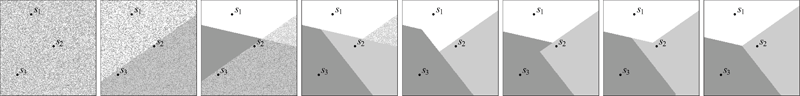
\includegraphics[width=16cm]{teaser}
\end{center}




% -------------------------------------------------------
\section*{Exercise 1 \rm Naive Algorithm}

 Use \textsc{DGtal} and \texttt{Image} data structure of
 \textsc{DGtal} to implement the naive algorithm as described above
 (see TP8).

Please consider a centroid data structure to store the position of the
$n$ centroids (maybe a \texttt{std::vector<RealPoint>}).

Start to experiment this algorithm on limited domains first.


\section*{Exercise 2 \rm Go Optimizations !}

In the description of the naive version, the random selection of a
pair of points/labels to swap. A first optimization can be described
as follows: For each label, we sort the points with respect to their
distance to its centroid (decreasing order).

Hence, we use this ordering to first try to swap points which are
farthest from their centroid. The argument is that farthest points
have an higher probability to be in the wrong ``cluster''.

This optimization would allow you to have faster convergence and thus
to be able to consider larger domains. In the authors' original
implementation,  several further tricks can be used, can you imagine
additional optimization heuristics.

\bibliographystyle{plain}
\bibliography{biblio}

\end{document}
